% !TEX root =  thesis.tex
\chapter{General System Requirements}\label{systemRequirements}

The MASS is designed as a domain independent central process where all domain knowledge is obtained from the SFI and CFI. To prevent any interference or assumption, the MASS and the Agents run as separate independent processes. The cTAEMS model supplies the internal knowledge used to build a Task Tree from which Agents will select available Methods for execution. This coupled with the easy configuration mechanism, logging, reporting and statistical analysis makes the simulator a good platform for research and evaluation of Multi-Agent Systems.

\section{System Features}

The following list offers a brief outline and description of the main features and functionalities of the MASS. The features are split into two major categories: core features and optional features. Core features are essential to the application's operation, whereas optional features are preferred but not required. For a better understanding of the basic features of the system see Figure 3.1.
%~\ref{fig:ERD}

\begin{figure}[H]
\centering
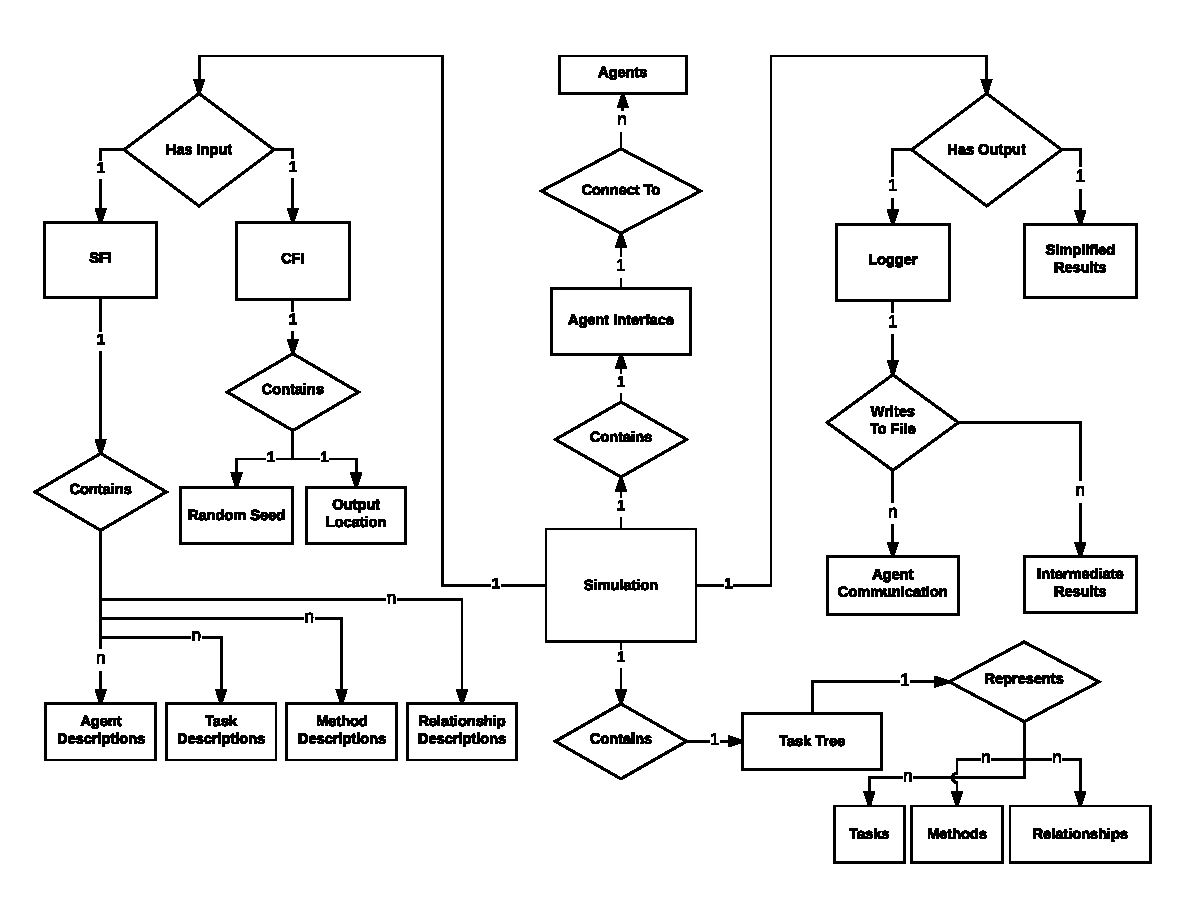
\includegraphics[width=6.5in]{figs/ERD.pdf}
\caption{ERD diagram for basic components of MASS.}
\label{fig:ERD }
\end{figure}

\begin{center} \textbf{Core Features} \end{center}

\begin{enumerate}

  \item\textbf{Running The MASS}: The MASS will run via the command line that optionally takes the SFI location as an input. If the SFI is not provided, the MASS will ask the user to specify its location. 
  
  \item\textbf{Simulation File Input (SFI)}: The SFI is a cTAEMS file.
    \begin{enumerate}
    \item The system is only required to support the use of the AND, OR, and SUM QAFs of the cTAEMS grammar.
    \item Methods and Tasks may only have Qualities and Durations. Costs will not be implemented.
    \item Excerpts of the grammar of a cTAEMS file are in Figures 3.2 and 3.3.
  \end{enumerate}

\begin{figure}
\begin{verbatim}
fragment Frag: ~('(' | ')');
Spaces:  (' ' | '\t')+;
fragment Label : '(' Spaces? 'label' Spaces? Frag*? ')' Spaces*?;
AgentToken :  '(' Spaces? 'spec_agent' Spaces Label? ')';
MethodToken :  '(' Spaces? 'spec_method' Spaces*? Label? Agent? Outcomes? ')';
\end{verbatim}
\caption{Excerpt of cTAEMS grammar to define a Method}
\label{fig:Grammar1}
\end{figure}

\begin{figure}[H]
\begin{verbatim}
fragment EarliestStartTime : '(' Spaces? 'earliest_start_time' Spaces? Frag*?
                    ')' Spaces*?;
fragment Deadline : '(' Spaces? 'deadline' Spaces? Frag*? ')' Spaces*?;
fragment Subtasks : '(' Spaces? 'subtasks' Spaces? Frag*? ')' Spaces*?;
fragment Qaf : '(' Spaces? 'qaf' Spaces? Frag*? ')' Spaces*?;
TaskToken :  '(' Spaces? 'spec_task' Spaces*? Label? EarliestStartTime?
                    Deadline? Subtasks? Qaf? ')';
\end{verbatim}
\caption{Excerpt of cTAEMS grammar to define a Task}
\label{fig:Grammar2}
\end{figure}
  
%\begin{figure}[H]
%\centering
%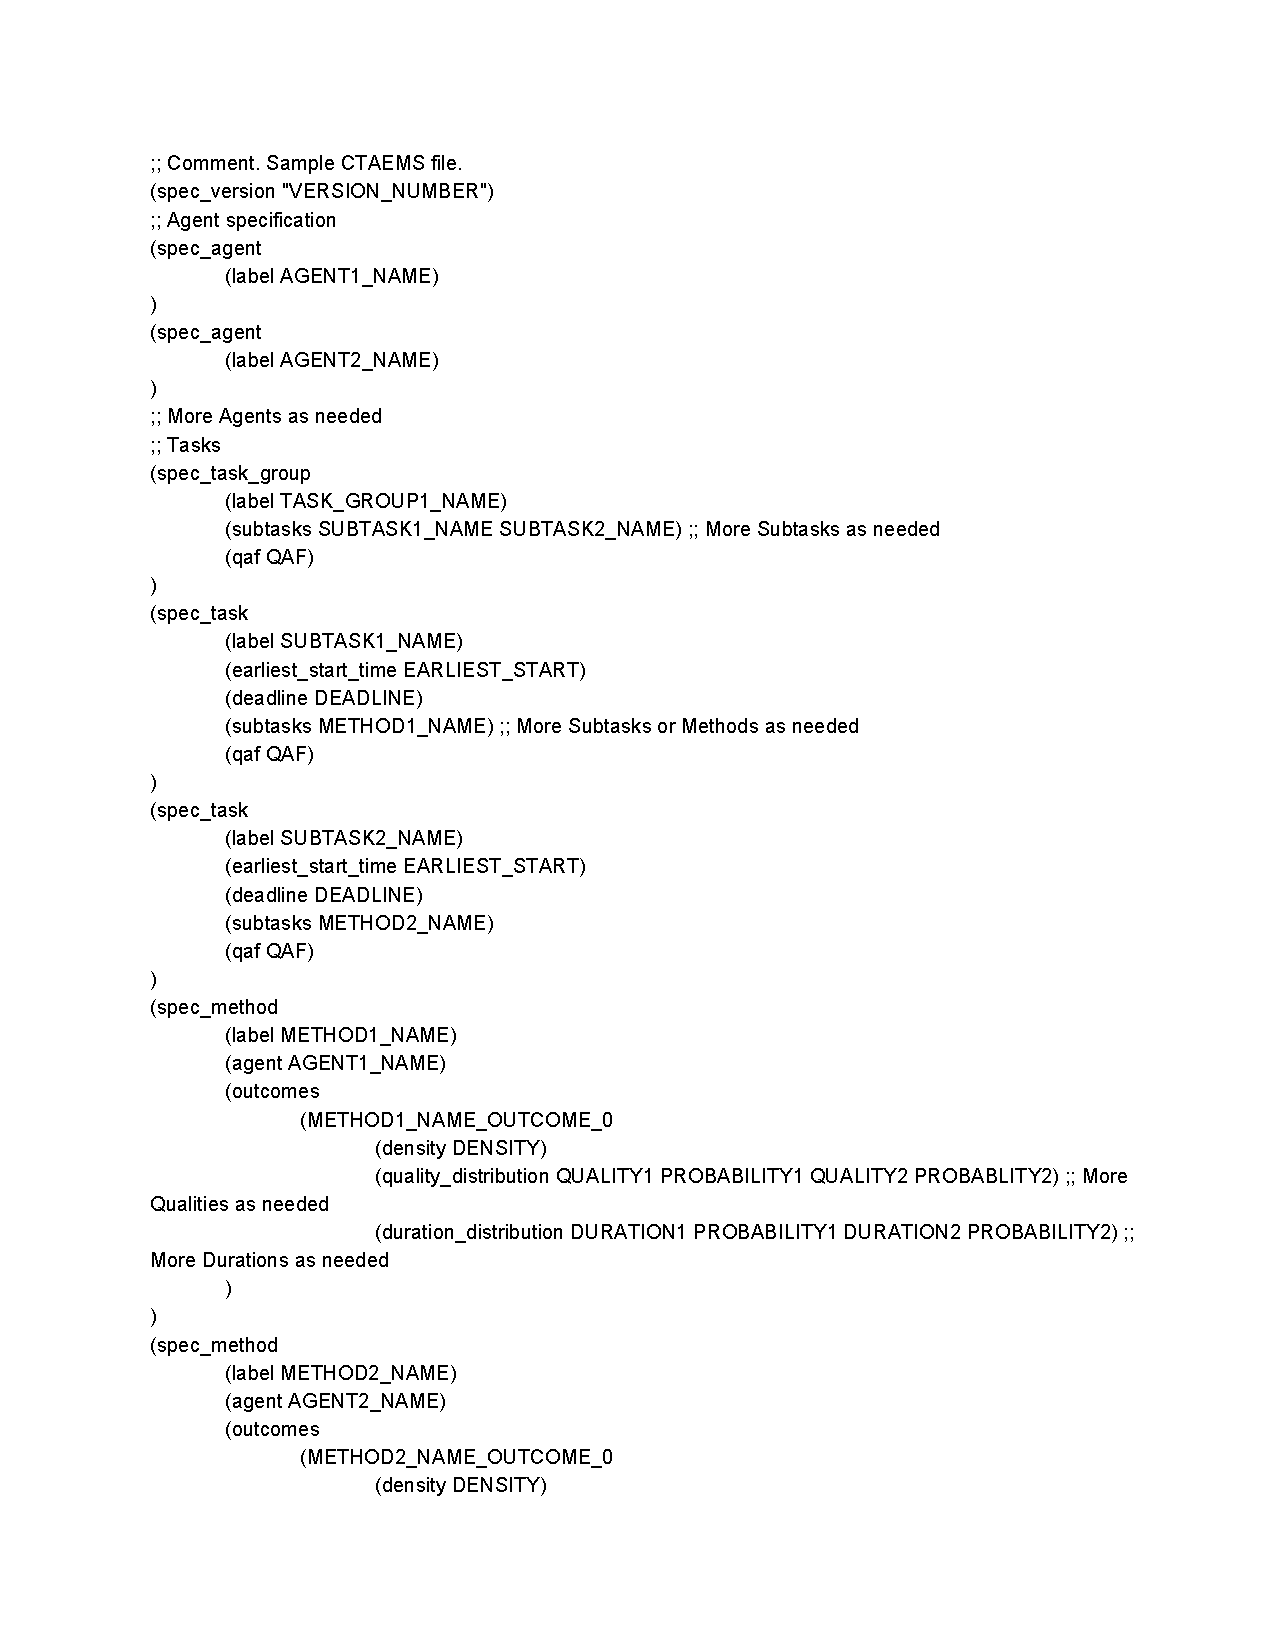
\includegraphics[trim=1.5cm 2cm 0cm 0cm, page=1, width=4.8in]{figs/cTAEMS.pdf}
%\caption{cTAEMS File Grammar part 1}
%\label{fig:cTAEMS}
%\end{figure}

%\begin{figure}[H]
%\centering
%\includegraphics[trim=0.5cm 15.5cm 0.5cm 0.5cm, page=2, width=4.8in]{figs/cTAEMS.pdf}
%\caption{cTAEMS File Grammar part 2}
%\label{fig:cTAEMS}
%\end{figure}
  
  \item \textbf{Configuration File Input (CFI)}: The program by default will look for a configuration file in the current directory named ``config.ini''.
  \begin{enumerate}
    \item If no configuration file is found the system will use default configuration values.
    \item The CFI will contain a random number seed, output file destination, the length (in milliseconds) of each Tick, and the port for the Simulator to listen on.
    \item Not all items in the CFI need to be specified. The system will resort to default values for the missing items.
    \item A sample CFI is shown in Figure 3.4.
  \end{enumerate}

\begin{figure}[H]
\centering
\texttt seed=8234827234\\
\texttt outputDestination=logs/\\
\texttt tickLength=1000\\
\texttt port=9876\\
\caption{Sample CFI}
\label{fig:CFI}
\end{figure}

%\begin{figure}[H]
%\centering
%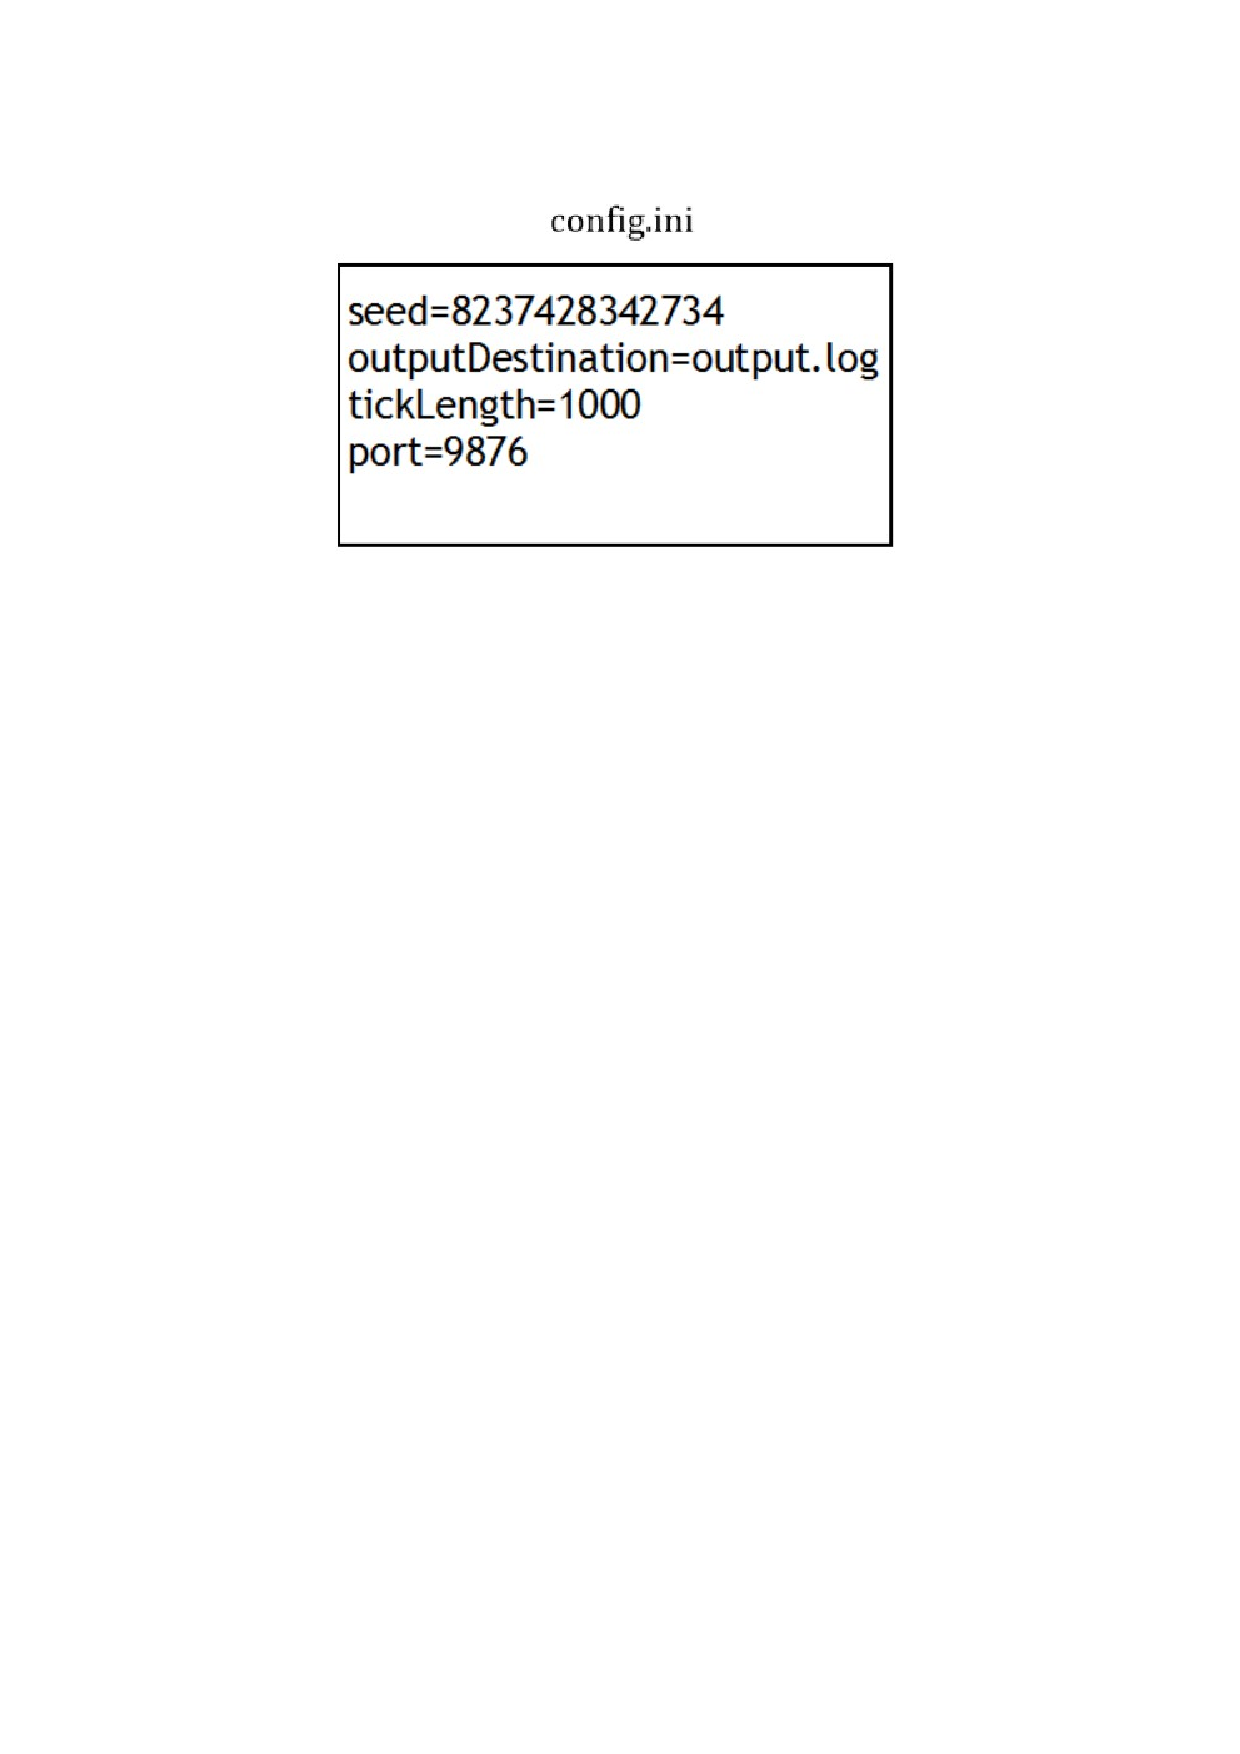
\includegraphics[trim=0cm 15cm 0cm 0cm,width=3in]{figs/CFI.pdf}
%\caption{Example CFI}
%\label{fig:CFI}
%\end{figure}
  
  \item\textbf{Agent Facing Interface}: The system will provide a consistent interface of which all Agents must implement in order to connect to the internal communication model.
  \begin{enumerate}
    \item All communication between the Agents and the MASS will be represented in the JSON format.
    \item The system must handle any Agent architecture in compliance with the Agent Interface (by using the correct JSON format of messages) and refuse connection to any Agent in violation of this. If an Agent doesn't use the correct format for JSON messages, the Simulator will terminate.
    \item It is the job of the agent to choose from the available Methods and report to the Simulation when starting and event.
    \item The Simulator will tell an agent when its Method has finished.
    \item Figures 3.5 - 3.18 describe the format of each Message type.
    \end{enumerate}
    
%\begin{figure}[H]
%\centering
%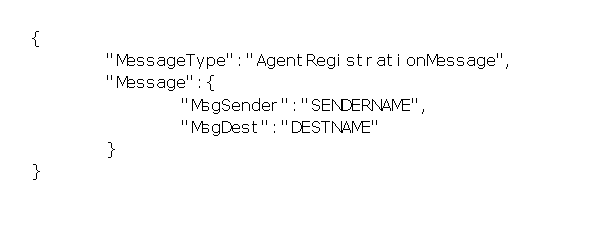
\includegraphics[width=3.6in]{figs/AgentRegistration.pdf}
%\caption{Format of AgentRegistration Message}
%\label{fig:AgentRegistration}
%\end{figure}

\begin{figure}[H]
\centering
\begin{verbatim}
                        {	
	                        "MessageType":"AgentRegistrationMessage",
 	                        "Message":{
 		                        "MsgSender":"SENDERNAME",
 		                        "MsgDest":"DESTNAME"
 	                        }
                        }
\end{verbatim}
\caption{Format of AgentRegistration Message}
\label{fig:AgentRegistration}
\end{figure}


\begin{figure}[H]
\centering
\begin{verbatim}
                        {	
                        	"MessageType":"AskMethodStatusMessage",
                         	"Message":
                         	{
                             "MsgSender":"SENDERNAME",
                             "MsgDest":"DESTNAME",
                             "MethodName":"METHODNAME"
	                        }
                        }
\end{verbatim}
\caption{Format of AskMethodStatus Message}
\label{fig:AskMethodStatus}
\end{figure}

\begin{figure}[H]
\centering
\begin{verbatim}
                        {
	                        "MessageType":"ConfirmMethodStartMessage",
 	                        "Message":
 	                        {
 	                        	"MsgSender":"SENDERNAME",
 	                        	"MsgDest":"DESTNAME",
 	                        	"MethodName":"METHODNAME",
 	                        	"Started":BOOLEAN
 	                        }
                        }
\end{verbatim}
\caption{Format of ConfirmMethodStart Message}
\label{fig:ConfirmMethodStart}
\end{figure}

\begin{figure}[H]
\begin{verbatim}
              {
                        "MessageType":"InitialTreeMessage",
                        "Message":{
                        "MsgSender":"SENDERNAME",
                        "MsgDest":"DESTNAME",
                        "Nodes":[(TASK|METHOD)+],
                        "Relationships":[(FACILITATES|HINDERS|ENABLES|DISABLES)*]
                        }
              }
              TASK {
                        "NodeType":"Task",
                        "NodeName":"NODENAME",
                        "QAF":"TASKQAF",
                        "EarlisetStartTime":"EARLIESTSTARTTIME",
                        "Deadline":"DEADLINE",
                        "VisibleToAgents":["AGENTNAME"+],
                        "SubTasks":["SUBTASKNAME"*]
              }
              METHOD {
                        "NodeType":"Method",
                        "NodeName":"NODENAME",
                        "AgentName":"AGENTNAME",
                        "Quality":DOUBLE,
                        "Duration":INTEGER,
                        "VisibleToAgents":["AGENTNAME"+]
              }
              FACILITATES | HINDERS {
                        "RelationshipType":"Facilitates" | "Hinders",
                        "RelationshipName":"RELATIONSHIPNAME",
                        "Source":"SOURCENAME",
                        "Destination":"DESTINATIONNAME",
                        "VisibleToAgents":["AGENTNAME"+],
                        "QualityFactor":DOUBLE,
                        "DurationFactor":DOUBLE
              }
              ENABLES | DISABLES {
                        "RelationshipType":"Enables" | "Disables",
                        "RelationshipName":"RELATIONSHIPNAME",
                        "Source":"SOURCENAME",
                        "Destination":"DESTINATIONNAME",
                        "VisibleToAgents":["AGENTNAME"+]
              }
\end{verbatim}
\caption{Format of InitialTree Message}
\label{fig:InitialTreeMessage}
\end{figure}

\begin{figure}[H]
\begin{verbatim}
              {
                        "MessageType":"UpdateTreeMessage",
                        "Message":{
                        "MsgSender":"SENDERNAME",
                        "MsgDest":"DESTNAME",
                        "Nodes":[(TASK|METHOD)+],
                        "Relationships":[(FACILITATES|HINDERS|ENABLES|DISABLES)*]
                        }
              }
              TASK {
                        "NodeType":"Task",
                        "NodeName":"NODENAME",
                        "QAF":"TASKQAF",
                        "EarlisetStartTime":"EARLIESTSTARTTIME",
                        "Deadline":"DEADLINE",
                        "VisibleToAgents":["AGENTNAME"+],
                        "SubTasks":["SUBTASKNAME"*]
              }
              METHOD {
                        "NodeType":"Method",
                        "NodeName":"NODENAME",
                        "AgentName":"AGENTNAME",
                        "Quality":DOUBLE,
                        "Duration":INTEGER,
                        "VisibleToAgents":["AGENTNAME"+]
              }
              FACILITATES | HINDERS {
                        "RelationshipType":"Facilitates" | "Hinders",
                        "RelationshipName":"RELATIONSHIPNAME",
                        "Source":"SOURCENAME",
                        "Destination":"DESTINATIONNAME",
                        "VisibleToAgents":["AGENTNAME"+],
                        "QualityFactor":DOUBLE,
                        "DurationFactor":DOUBLE
              }
              ENABLES | DISABLES {
                        "RelationshipType":"Enables" | "Disables",
                        "RelationshipName":"RELATIONSHIPNAME",
                        "Source":"SOURCENAME",
                        "Destination":"DESTINATIONNAME",
                        "VisibleToAgents":["AGENTNAME"+]
              }
\end{verbatim}
\caption{Format of UpdateTree Message}
\label{fig:UpdateTreeMessage}
\end{figure}

\begin{figure}[H]
\centering
\begin{verbatim}
                        {
	                        "MessageType":"NotifyMethodCompletedMessage",
 	                        "Message":
 	                        {
 	                        	"MsgSender":"SENDERNAME",
 	                        	"MsgDest":"DESTNAME",
 	                        	"MethodName":"METHODNAME",
 	                        	"Quality":DOUBLE,
 	                        	"Duration":INTEGER
 	                        }
                        }
\end{verbatim}
\caption{Format of NotifyMethodCompleted Message}
\label{fig:NotifyMethodCompleted}
\end{figure}

\begin{figure}[H]
\centering
\begin{verbatim}
                        {
	                        "MessageType":"NotifyMethodStatusMessage",
 	                        "Message":
 	                        {
 	                        	"MsgSender":"SENDERNAME",
 	                        	"MsgDest":"DESTNAME",
 	                        	"MethodName":"METHODNAME",
 	                        	"Started":BOOLEAN,
 	                        	"Completed":BOOLEAN,
 	                        	"Enabled":BOOLEAN
 	                        }
                        }
\end{verbatim}
\caption{Format of NotifyMethodStatus Message}
\label{fig:NotifyMethodStatus}
\end{figure}

\begin{figure}[H]
\centering
\begin{verbatim}
                       {
	                       "MessageType":"NotifyRelationshipActivationMessage",
 	                       "Message":
 	                       {
 	                       	"MsgSender":"SENDERNAME",
 	                       	"MsgDest":"DESTNAME",
 	                       	"RelationshipName":"RELATIONSHIPNAME"
 	                       }
                       }
\end{verbatim}
\caption{Format of NotifyRelationshipActivation Message}
\label{fig:NotifyRelationshipActivation}
\end{figure}

\begin{figure}[H]
\centering
\begin{verbatim}
                        {
	                        "MessageType":"SetRandomSeedMessage",
 	                        "Message":
 	                        {
 	                        	"MsgSender":"SENDERNAME",
 	                        	"MsgDest":"DESTNAME",
 	                        	"Seed":LONG
 	                        }
                        }
\end{verbatim}
\caption{Format of SetRandomSeed Message}
\label{fig:SetRandomSeed}
\end{figure}

\begin{figure}[H]
\centering
\begin{verbatim}
                        {
                        	"MessageType":"StartMethodMessage",
                         	"Message":
                         	{
 	                        	"MsgSender":"SENDERNAME",
 	                        	"MsgDest":"DESTNAME",
 	                        	"MethodName:"METHODNAME"
 	                        }
                        }
\end{verbatim}
\caption{Format of StartMethod Message}
\label{fig:StartMethod}
\end{figure}

\begin{figure}[H]
\centering
\begin{verbatim}
                        {
                        	"MessageType":"StartSimulationMessage",
                         	"Message":
                         	{
 	                        	"MsgSender":"SENDERNAME",
 	                        	"MsgDest":"DESTNAME",
 	                        }
                        }
\end{verbatim}
\caption{Format of StartSimulation Message}
\label{fig:StartSimulation}
\end{figure}

\begin{figure}[H]
\centering
\begin{verbatim}
                        {
                        	"MessageType":"EndSimulationMessage",
                         	"Message":
                         	{
 	                        	"MsgSender":"SENDERNAME",
 	                        	"MsgDest":"DESTNAME",
 	                        }
                        }
\end{verbatim}
\caption{Format of EndSimulation Message}
\label{fig:EndSimulation}
\end{figure}

\begin{figure}[H]
\centering
\begin{verbatim}
                        {
                        	"MessageType":"NextTickMessage",
                         	"Message":
 	                        {
 	                        	"MsgSender":"SENDERNAME",
 	                        	"MsgDest":"DESTNAME",
 	                        	"Tick":LONG
 	                        }
                        }
\end{verbatim}
\caption{Format of NextTick Message}
\label{fig:NextTick}
\end{figure}

\begin{figure}[H]
\begin{verbatim}
                        {
                        	"MessageType":"AgentToAgentMessage",
                        	"Message":
                        	{
                        		 "MsgSender":"SENDERNAME",
                        		 "MsgDest":"DESTNAME",
                        		 "Content":JSONOBJECT
                        	}
                        }
\end{verbatim}
\caption{Format of AgentToAgent Message}
\label{fig:AgentToAgentMessage}
\end{figure}
    
    
    \item\textbf{Agent Communication}: Agents must have the ability to communicate throughout the Simulation.
    \begin{enumerate}
    \item An Agent can send a message intended for another Agent, or it can send one directly to the Simulator. Either way, the message will pass through the Simulator so that it may log the communication patterns of the Agents.
  \end{enumerate}
  
  \item\textbf{Task Tree}: A Simulation will consist of a Task Tree that keeps track of what Methods are able to be executed at any given time.
   \begin{enumerate}
    \item The Task Tree consists of Tasks and Methods. Tasks can have Nodes as children while Methods are the leaves of the tree. The total quality of a Task Group is determined from the head of that group's Task Tree.
    \item When a Method is finished, it's quality will propagate up through the tree based on its parents' QAFs.
    \item An example Task Tree showing three Tasks, four Methods, and two Relationships is shown in Figure 3.19.
  \end{enumerate}

\begin{figure}[H]
\centering
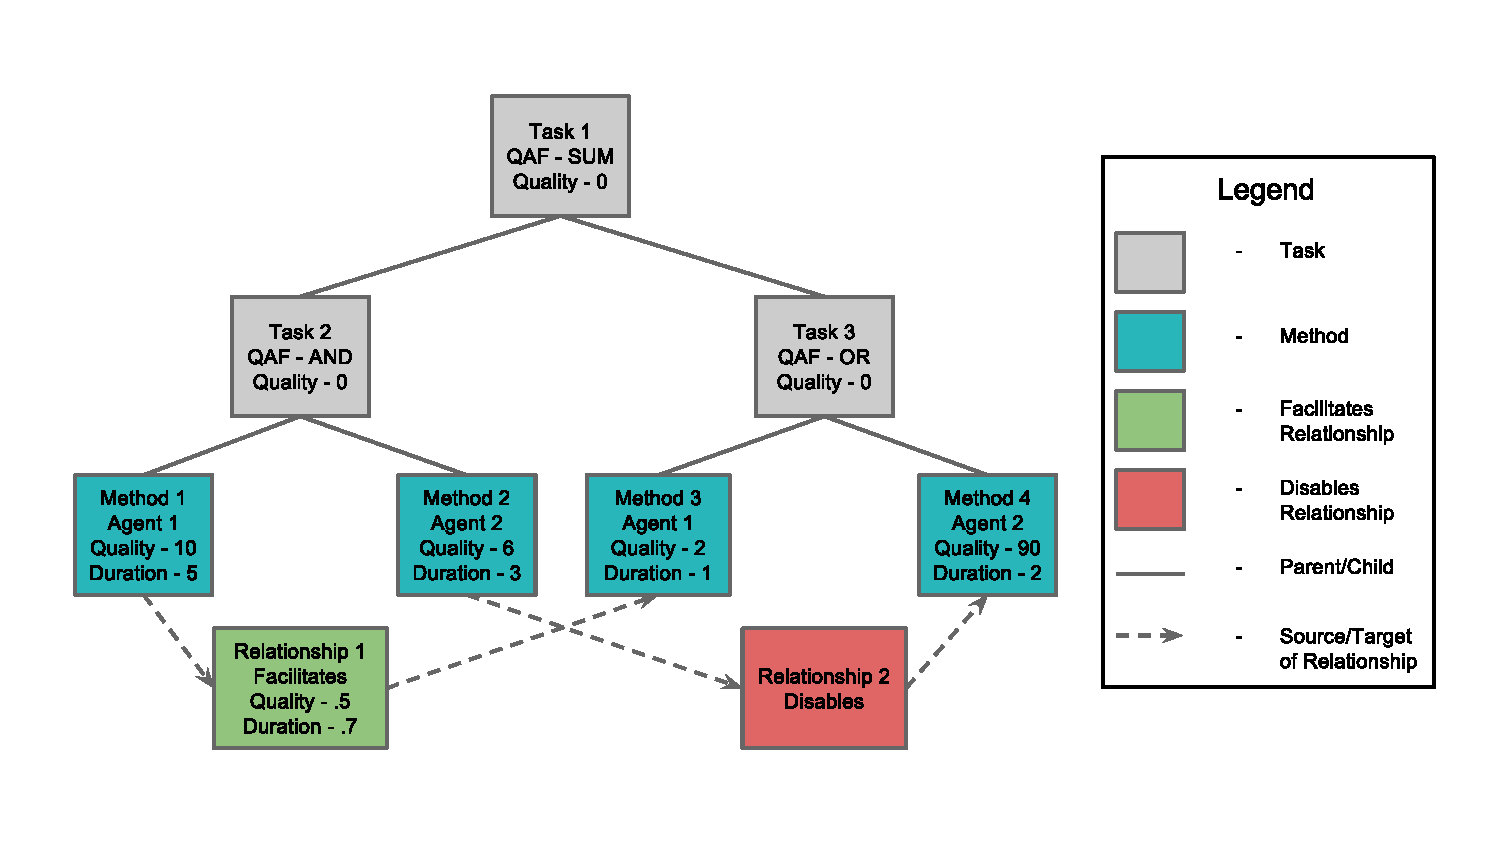
\includegraphics[width=6.5in]{figs/TaskTree.pdf}
\caption{Example Task Tree with Relationships}
\label{fig:TaskTree}
\end{figure}
  
  \item\textbf{Creating a Simulation}: A Simulation must be repeatable.
   \begin{enumerate}
    \item Any probability distributions must be computed using the seed value obtained from the CFI as the SFI is being parsed.
    \item Agents must be given the seed value obtained from the CFI in case they use any random calculations in their logic.
    \item Agents are given an initial set of Nodes that are visible to them at the start of the Simulation. Visibility is defined as follows:
    	\subitem An Agent can see its assigned Methods.
    	\subitem An Agent can see all Tasks that are direct ancestors of its Methods.
    	\subitem An Agent can see all Relationships that have one of the Agent's visible Nodes as the source/target.
    	\subitem An Agent can see the Nodes that are the sources/targets of one of that Agent's visible Relationships.
    \item When any Node or Relationship is visible to an Agent, that Agent knows:
    	\subitem The name of the Node or Relationship
    	\subitem The names of all other Agents that can see that Node
    \item When a Method is visible to an Agent, that Agent knows:
   	\subitem The Method's quality
	\subitem The Method's duration
    \item When a Task is visible to an Agent, that Agent knows:
   	\subitem The Task's QAF
   	\subitem The Task's (visible) Subtasks
    \item When a Relationship is visible to an Agent, that Agent knows:
    	\subitem The type of the Relationship
    	\subitem The source and target of the Relationship
    	\subitem The new quality and duration if the Relationship is of Facilitates or Hinders type
  \end{enumerate}
  
  \item\textbf{Running a Simulation}: The MASS must keep track of Nodes.
    \begin{enumerate}
    \item The MASS must know what Methods are able to be executed at any given time.
    \item The MASS must know what Methods are being executed at any given time.
    \item The MASS must know what Methods have been executed at any given time.
    \item The MASS must know what the Qualities of all Tasks are at any given time.
    \item The MASS must know which Tasks have been completed at any given time.
    \item The MASS must know when the Simulation is finished. This is achieved when every Task Group has no Methods that are both enabled and unfinished.
  \end{enumerate}
  
  \item\textbf{Simulation Output}: The system will produce an output detailing the overall Quality and Duration of the entire Simulation.
  \begin{enumerate}
  \item The output should occur on the command line.
  \end{enumerate}
  
  \item\textbf{Log File Output (LFO)}: The system will produce a detailed log file including the intermediate Quality and Cost between every Task and Method.
  \begin{enumerate}
  \item The LFO will contain a transcript of Agent communication
  \item The LFO will contain compiled statistics on Agent communication frequency.
  \item The LFO will contain the intermediate and final Quality, and Duration that results from completing an Event in the Task Tree.
  \end{enumerate}

\end{enumerate}


\begin{center} \textbf{Additional Features} \end{center}

This is a short list of features that will be added to the MASS if time permits. If they are to be added, they will move into the full system requirements.

\begin{enumerate}

\item\textbf{Graphical Representation of Task Tree}:  The Task Tree is a hierarchical tree-like structure representing Nodes and the Relationships between them.
\begin{enumerate}
\item The system may represent this structure as a graphical model to help understand the Simulation results better. 
\end{enumerate}

\item\textbf{cTAEMS Grammar Support}: The system may go beyond the logical AND, OR, and SUM operations and include additional implementations within the cTAEMS grammar.

\item\textbf{Agent Behavior}: The System may support the ability of Agents to stop, pause, or resume Methods if such actions are applicable based on the Simulation specifications. 

\end{enumerate}
